%!TEX root = ../SciVis.tex
Height plots are a visualization technique that create a three dimensional representation of a scalar datasets. Transforming a 2D-scalar dataset  into  topological surface is straightforward. We construct the surface by using a triangle strip, while the height of each vertex is determined by the linearly scaled scalar value. In fact the value will be scaled between 0 and \verb|max height|, in this case 100px. 

In order to display the height plot correctly, we must switch from a parallel projection to a perspective projection that is capable of displaying depth. 
We set up our scene by using \verb|gluPerspective| and the camera by using \verb|gluLookAt|. In addition, enabled lightning and smooth shading.
 
Smooth shading requires normals at every vertex normals, which can be computed by averaging the surface normals of all planes adjacent to a vertex. Figure~\ref{fig:figures_heightplot_normalization} shows the six surface normals that are used to calculate a vertex normal.
The surface normals can be obtained from the data by using the four vertices of a cell two construct two vectors for each triangular surface. Using the cross-product of these two vectors returns a vector that will perpendicular to the surface - the normal. However, it has to be checked wether the normal is facing inwards or outwards (towards the visible front or invisible back).  Figure~\ref{fig:heighplot_densityNormals} shows the calculated normals for each vertex. It can be seen that the vertex normal is influenced by the orientation of the adjacent surfaces. 

\begin{figure}[htbp]
\centering
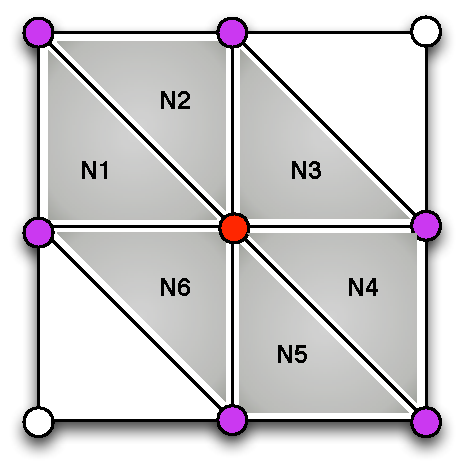
\includegraphics[height=3in]{figures/heightplot/normalization.pdf}
\caption{In order to calculate the vertex normal (red), the surface normals of the adjacent triangles are averaged.}
\label{fig:figures_heightplot_normalization}
\end{figure} 


We implemented a simple keyboard-based mechanism to modify the perspective with the arrow-keys and other special keys. First of all, the whole scene can be tilted by a rotation around the x-axis. This gives the user the possibility to influence the angle in which he looks at the scene (from the top or front). Furthermore, it is possible to change the direction of the camera on an xy-plane and to adjust the distance of  camera  from the scene. 


\begin{figure}[htbp]
\centering
\begin{minipage}[t]{0.48\textwidth}
        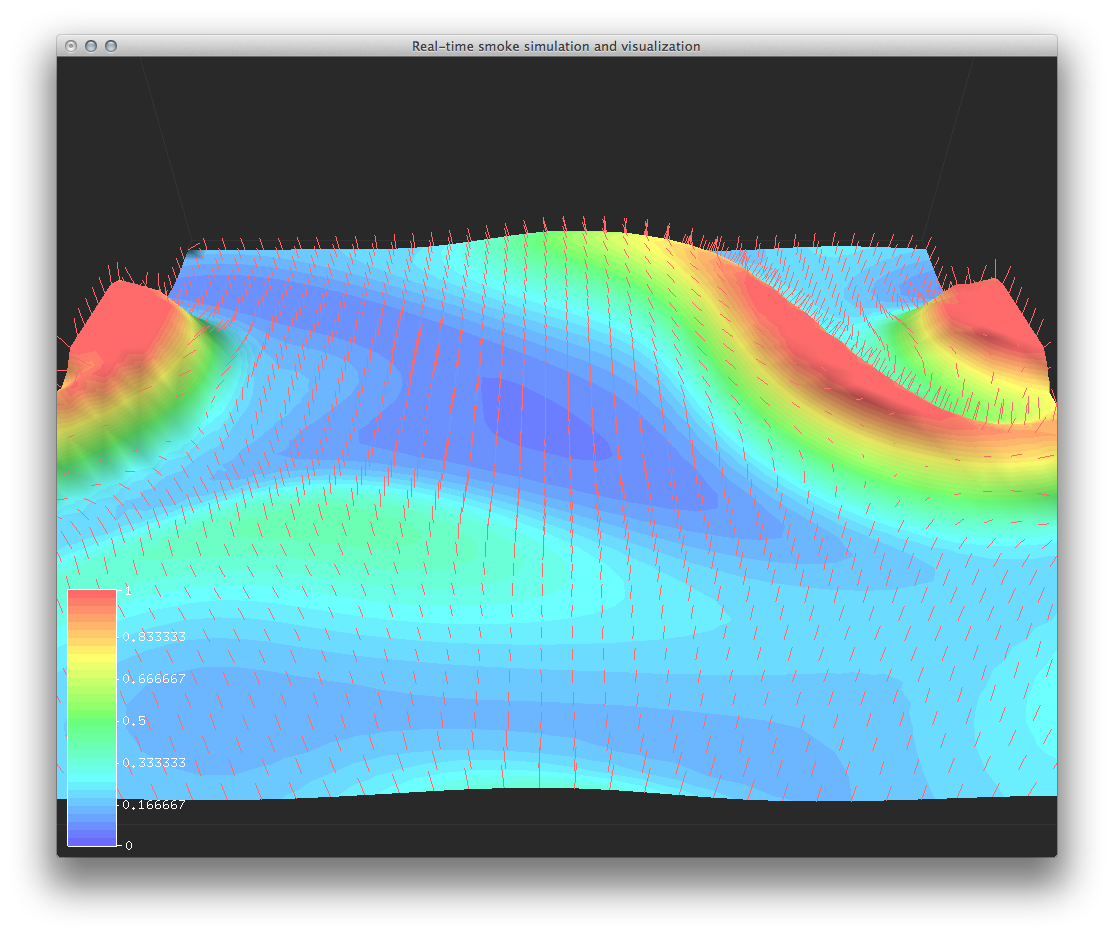
\includegraphics[height=3in]{figures/heightplot/densitynormals.png}
        \caption{The height plot and colormap both shows the density. The calculated vertex normals are shown as little red pikes facing into the direction of the normal.}
\label{fig:heighplot_densityNormals}
\end{minipage}\hspace{.04\textwidth}%
\begin{minipage}[t]{0.48\textwidth}
 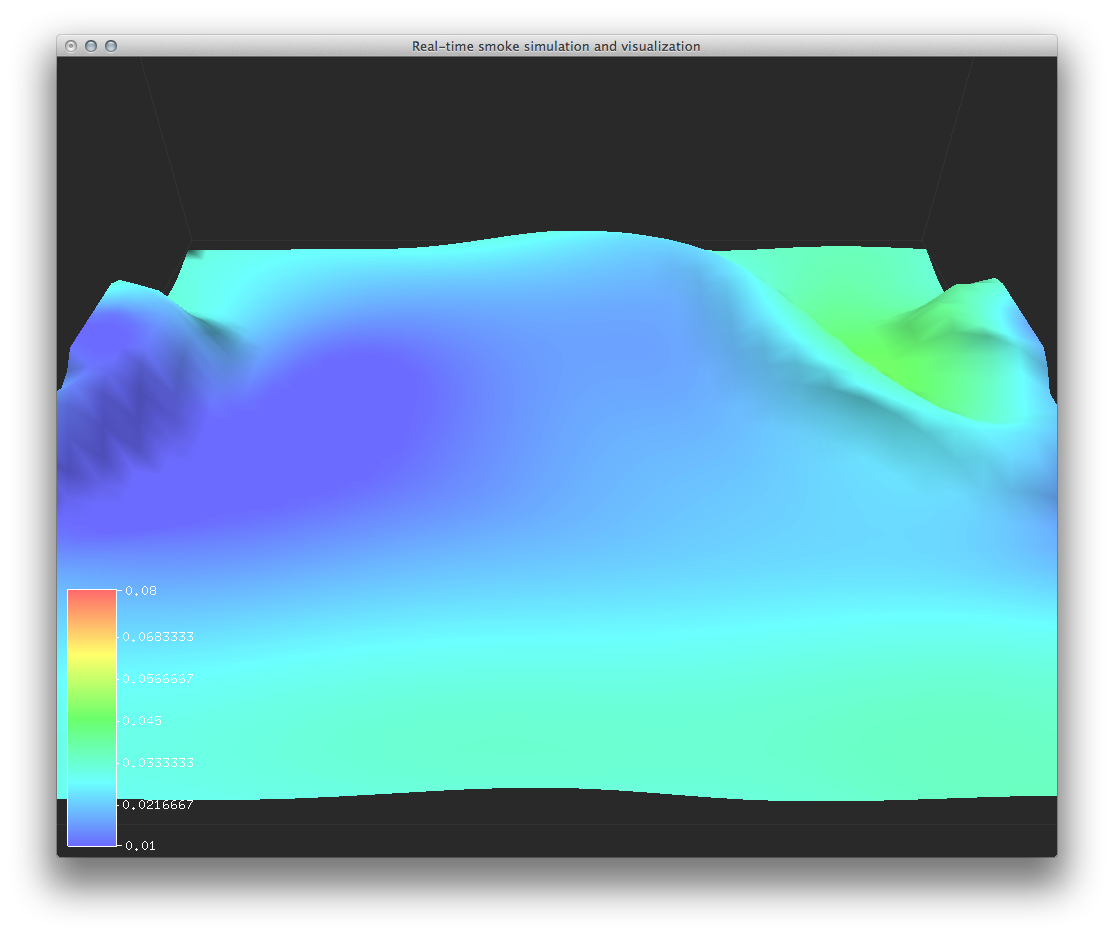
\includegraphics[height=3in]{figures/heightplot/densityvelocity.png}
    \caption{The height plot shows density while the colormap visualizes the velocity. It can be seen that the topological peaks and color peaks are not aligned }
    \label{fig:heighplot_densityVelocity}
\end{minipage}
\end{figure}


The height plot is able to visualize two scalar datasets at once. The first dataset is encoded in the height and the second one in the color of the surface. The datasets can be selected in the user interface and it is also possible to specify whether the values should be clamped within a predefined range or scaled according to the local maximum and minimum. 
We use the same mechanism to map scalar-values to color that has been described in the color mapping step. Basically, all options that are available to influence the colormap visualization in 2D are also possible in 3D. Reducing the number of colors will make it easier for the user to compare the height of different peaks and valleys. However, this will reduce the accuracy of the inverse mapping step as the user is not able to see all values but only certain ranges (cf. Figure~\ref{fig:figures_heightplot_densitydensitybanding}).


As illustrated in Figure~~\ref{fig:heighplot_densityVelocity},it is important to choose the colormap carefully as the colormap creates an artificial shaded topology that does not correlate with the actual height plot and thus might be confusing or unintuitive.

\begin{figure}[htbp]
    \centering 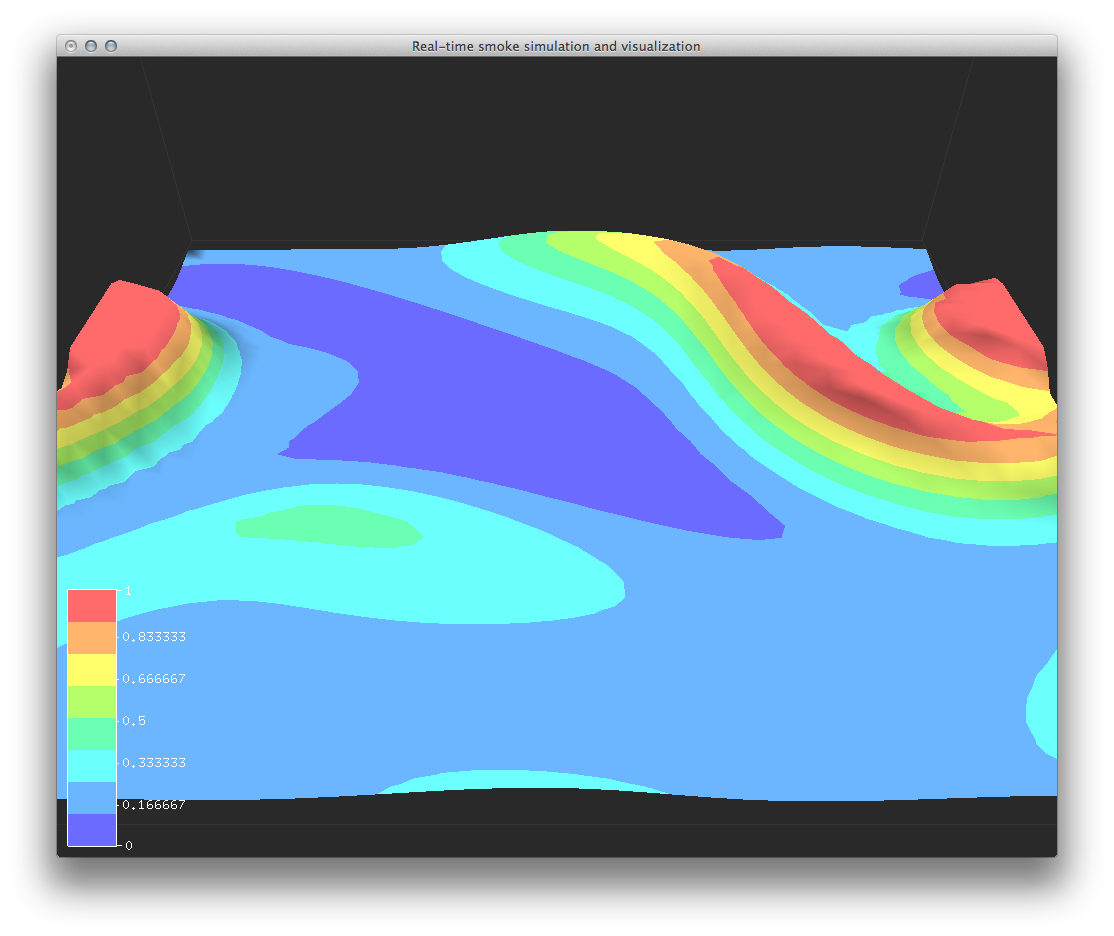
\includegraphics[height=3in]{figures/heightplot/densitydensitybanding.png}
    \caption{Reducing the number of colors makes it easy to compare the height of different peaks but it comes at the cost of a less accurat inverse mapping.}
    \label{fig:figures_heightplot_densitydensitybanding}
\end{figure}



